\documentclass[11pt,letterpaper]{article}

\usepackage{natbib}
%\usepackage{cite}
\usepackage{graphicx}
\usepackage[margin=1.in,centering]{geometry}
\usepackage{hyperref}
\usepackage{caption}
\usepackage[export]{adjustbox}
\usepackage{float}

\newcommand{\mnras}{MNRAS}
\newcommand{\apj}{ApJ}
\newcommand{\aapr}{A\&ARv}

\begin{document}

\title{Optical/UV Band
Reverberation Mapping of NGC 5548 with Frequency-Resolved Techniques}

\author{Otho A. Ulrich,$^{1,2}$ Edward M. Cackett$^{1}$
\\
% List of institutions
$^{1}$Department of Physics and Astronomy, Wayne State University\\
$^{2}$Department of Physics, Western Michigan University\\
}
\date{August 8, 2016}

\maketitle

\begin{abstract}

Power spectral densities and time delays of 19 wavelength bands are recovered as part of a reverberation mapping of NGC 5548. The latest time-variable light curves are made available in STORM III by \cite{2016ApJ...821...56F}. The uneven distribution of flux data in those curves necessitates the use of a maximum likelihood method in conjunction with Fourier transformations to produce the frequency-dependent values of interest. Variability in the emissions is confirmed in the power spectral densities, and the time delays show the expected frequency dependence. The time delays also appear to have wavelength dependence. There are issues computing accurate error estimates for both distributions that remain as yet unresolved. The transfer function should be recoverable once those and any additional computational issues are resolved.

\end{abstract}

\section{Introduction}

The local Type-I Seyfert galaxy NGC 5548, while perhaps the best-studied active galaxy, remains an object of intense interest and study to modern astronomy. Direct observation of active galactic nuclei (AGN) such as that thought to exist at the center of NGC 5548 is rarely possible. The astronomer may infer the properties of AGN from the dynamics of their variable spectra. \cite{2016ApJ...821...56F} published the most complete set of time-dependent light curves yet collected from an active galactic nucleus as part III of STORM, an extensive optical/UV observational campaign carried out on NGC 5548. We now attempt to use frequency-domain analyses to map the reverberation in the observed light curves.

\section{Reverberation Mapping}
	One model for AGN suggests that a hot accretion disk is incident upon a central super-massive black hole (SMBH). Electromagnetic emission emergent from the gas surrounding the SMBH is reprocessed by the disk, resulting in observed response delays between emission peaks. If the temperature of the disk decreases radially from the SMBH, the observed time delays can be expected to increase with decreasing wavelength. Furthermore, as the emissions are reprocessed in the disk, they become blurred, so the variability can be expected to decrease with wavelength. A transfer function encodes the geometry of the system by describing the time-dependent response of each light curve against the others. Recovering the function from the observed light curves is a primary goal of reverberation mapping.

	This technique has become a standard for calculating the black hole mass of AGN. It is well-described by \cite{2007MNRAS.380..669C} and \cite{2014A&ARv..22...72U} and many others. It continues to be refined, and may also become a tool to measure the black hole spin of these systems (\cite{2016arXiv160606736K}).

	\begin{figure}
		\centering
		\includegraphics[width=3.5in]{../img/basic_geometry.png}
		\caption{Simple geometry of reverberation in the accretion disk. Some continuum emissions are reprocessed before escaping toward the observer.}
	\end{figure}

\subsection{Frequency-domain Analysis}

	The transfer function $g(t)$ is related to two light curves as being convoluted against the reference light curve (\ref{time_transfunc}). The convolution theorem provides that convolution in the time domain is equivalent to pointwise multiplication in the frequency domain (\ref{freq_transfunc}). The transfer function therefore lends itself well to frequency-domain analyses.

	\begin{equation}
		\label{time_transfunc}
		y(t) = \int_{-\infty}^{\infty} g(\tau) x(t-\tau)  {\rm d}\tau
	\end{equation}

	\begin{equation}
		\label{freq_transfunc}
		Y(\nu) = G(\nu) X(\nu)
	\end{equation}

    The power spectral density (PSD) provides a measure of the variability of the flux in a band. It is defined as $|X(\nu)|^2 = X^*(\nu)X(\nu)$, where $^*$ denotes the complex conjugate, and can be produced using Fourier transforms. The transfer function is therefore related to the PSD of two light curves:

    \begin{equation}
        |Y(\nu)|^2 = |G(\nu)|^2 |X(\nu)|^2
    \end{equation}

    Given two bands, a cross spectrum can also be computed. The cross spectrum is defined as $C(\nu) = X^*(\nu) Y(\nu)$. The argument $\phi$ of the cross spectrum is the phase lag between the two signals. The time delay $\tau$ can therefore be computed from the cross spectrum using
    
    \begin{equation}
        \tau(\nu) = \frac{\phi(\nu)}{2\pi\nu}
    \end{equation}

    Given equation \ref{freq_transfunc}, the cross spectrum can be written as
        
    \begin{equation}
        C(\nu) = X^*(\nu) G(\nu) X(\nu) =  G(\nu) |X(\nu)|^2 
    \end{equation}

    The time delays are therefore trivially predicted as a function of frequency from the cross spectrum. The frequency dependence of these lags in turn relates directly to the transfer function. Very good explanations of these techniques and the associated mathematics are available from \cite{2014A&ARv..22...72U}.

    \subsection{Tophat Transfer Function}

	A tophat function provides a simple model of the impulse response of a delayed light curve. A fast Fourier transform method of this impulse response provides the time delay spectrum as a function of temporal frequency. This simple model provides a guideline for how the computed time delays are expected to be distributed as a function of frequency. Once the time delays are extracted from the observational datasets, they might be fitted with a tophat function, however, a more complicated function such as a log-Gaussian function is probably more appropriate.

    \begin{figure}
        \centering
        \begin{minipage}{.475\textwidth}
            \centering
            \includegraphics[width=1\linewidth]{../img/tophat_timedomain.pdf}
            \captionof{figure}{Tophat functions in the time domain show an average time delay of the reverberating curve and a constant distribution in time over an interval. An area of unity indicates no loss of signal in the response.}
            \label{fig:th_time}
        \end{minipage}
        \hfill
        \begin{minipage}{.475\textwidth}
            \centering
            \includegraphics[width=1\linewidth]{../img/tophat_freqdomain.pdf}
            \captionof{figure}{The time delays associated with each tophat function. Distinct features related to the average time lag are present (maximum, value of $\nu$ at steepest change), and complicated relationships with higher frequency waves can be noted.}
            \label{fig:th_freq}
        \end{minipage}
    \end{figure}


	\subsection{Unevenly-Sampled Data}

    Traditional frequency-domain analyses require data that is evenly sampled. Due primarily to weather, optical reverberation mapping datasets generally contain unevenly sampling. Because of this, until now, optical reverberation mapping has been limited mainly to time-domain analyses, e.g., cross-correlation. While it can handle datasets with significant sampling-variability, cross-correlation is only able to determine the average time lag for a given light curve; however, more information is contained within the light curves than just their average time lag.

    Some X-ray datasets contain gaps due to orbital mechanics, which motivated the work by \cite{2013ApJ...777...24Z}, where a maximum likelihood method is used to perform Fourier analysis on light curves with gaps. Since its development, this technique has found success among studies of observations captured by low-orbit X-ray telescopes that exceed the telescopes' orbital periods, such as the analysis performed by \cite{2016arXiv160606736K}. This technique is now being applied to the optical datasets published in STORM III. If successful, it may provide new insight into the reverberations present in the accretion disk and other structures of the nucleus in NGC 5548.
 	
\section{Analysis}

\cite{2016ApJ...821...56F} published the best dynamic data yet collected from NGC 5548 over a 260-day period, for 19 bands throughout the optical and into the UV domains. These data were collected from a variety of observatories, including both space and ground-based telescopes, and thus have significantly uneven and variable sampling rates. The 1367\AA$ $ light curve, obtained from observations made with the Hubble Space Telescope, is chosen as the reference curve. The power spectral densities and time delays as a function of temporal frequency are computed for each band in the dataset -- 18 bands not including the reference band.

In STORM III, a reverberation mapping analysis is performed using cross-correlation to find the average time delay for each wavelength. These results are compared to a number of possible models, however, the average time lag leaves a lot of uncertainty when trying to constrain an appropriate model. More information is contained in the light curves, and a frequency-domain analysis should provide better constraints.

\begin{figure}
    \centering
    \begin{minipage}{.475\textwidth}
        \centering
        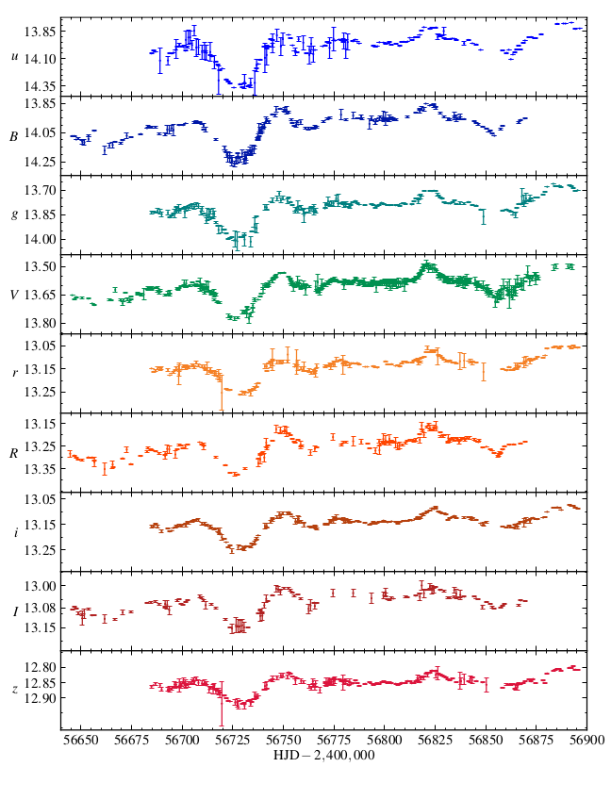
\includegraphics[width=1\linewidth]{../img/lightcurves.pdf}
        \captionof{figure}{Data published by \cite{2016ApJ...821...56F} in STORM III shows highly-variable light curves with significantly uneven sampling.}
        \label{fig:lightcurves}
    \end{minipage}
    \hfill
    \begin{minipage}{.475\textwidth}
        \centering
        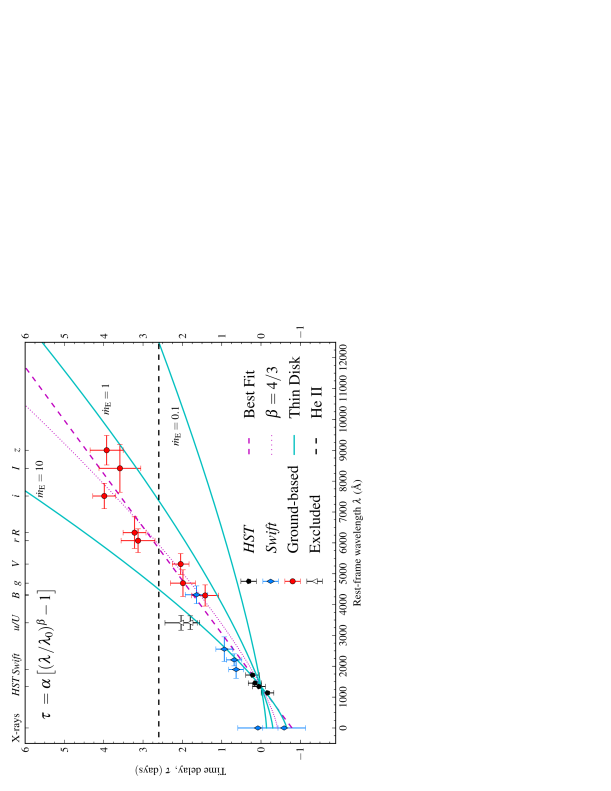
\includegraphics[width=1\textwidth]{../img/TCCF_fausnaugh.pdf}
        \captionof{figure}{Cross-correlation analysis of lightcurves presented by \cite{2016ApJ...821...56F} compared average time lags to AGN structure models.}
        \label{fig:cc_analysis}
    \end{minipage}
\end{figure}


The light curves analysed here are unevenly distributed along the time axis, which suggests that the maximum likelihood method developed by \cite{2013ApJ...777...24Z} is a reasonable candidate for analysing these data by producing the PSD and time delays. The latest version as of July, 2016, of the C++ program "psdlag" associated with that work is used to directly produce the PSD and cross spectra. The time delay spectrum is produced from the cross spectrum by dividing it by $2 \pi f$, with $f$ the mean frequency for a given bin.

\begin{figure}
    \centering
    \begin{minipage}{.475\textwidth}
        \centering
        \includegraphics[width=1\linewidth]{../img/PSD_1367Å_{σ∊CM}.pdf}
        \captionof{figure}{Power spectral density for 1367\AA, the chosen reference band.}
        \label{fig:psd_1367}
    \end{minipage}
    \hfill
    \begin{minipage}{.475\textwidth}
        \centering
        \includegraphics[width=1\linewidth]{../img/timelag_1367Å_≺_7647Å_{σ∊CM}.pdf}
        \captionof{figure}{The time delay computed from the cross spectrum of 7647\AA and 1367\AA.}
        \label{fig:timelag_7647}
    \end{minipage}
\end{figure}


	\subsection{Errors}
	For the presented set of resultant data, the error estimates are extracted from the covariance matrix. This method assumes that the errors between frequency bins are not correlated, so these values only represent a lower limit of the true variability. Scanning the likelihood function can provide better error estimates at the cost of computation time, as can running Monte Carlo simulations. All of these methods are built into the "psdlag" program provided by \cite{2013ApJ...777...24Z}.

    An error analysis by scanning the likelihood function was attempted, but this analysis was plagued by computational issues that prevented some models from properly optimizing. Monte Carlo simulations were also attempted as a way of estimating the variability of the resultant values. Many errors obtained from this method were larger than the expected accurate values. Therefore, this analysis was also excluded. The ultimate goal is to use one of these more accurate methods, and the errors currently reported should be considered temporary and unreliable.

    \subsection{Results}
    \label{results}

    In figure \ref{psd_atlas}, an atlas of the power spectral densities for all 18 reverberated bands is provided. Figure \ref{timelag_atlas} provides the time delay spectra for each band. The reference band PSD is provided separately. Producing the time delay map is a significant step toward recovering the transfer function.

    \begin{figure}
        \centering
        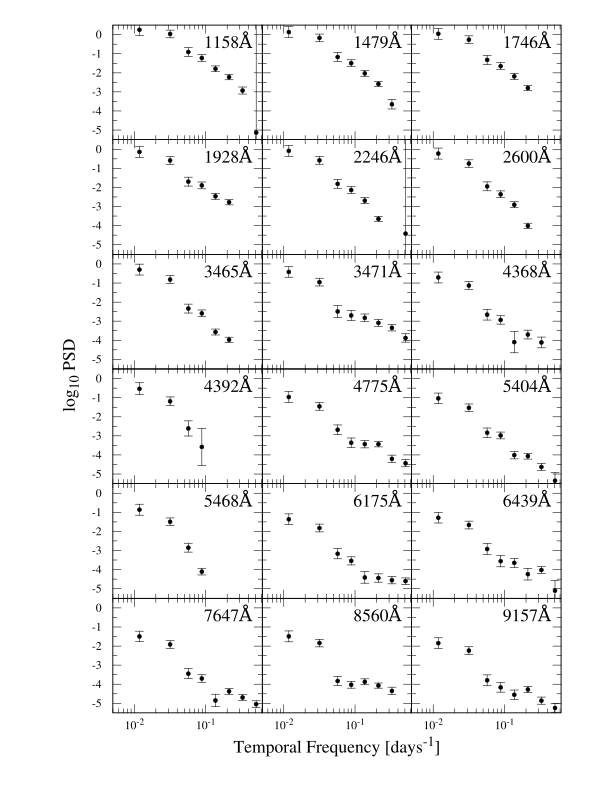
\includegraphics[width=.9\textwidth]{../img/psd_atlas.pdf}
        \caption{Power spectral densities for all observed light curves, excluding the reference curve. The decrease in variability with increasing wavelength is in agreement with that prediction.}
        \label{psd_atlas}
    \end{figure}

    \begin{figure}
        \centering
        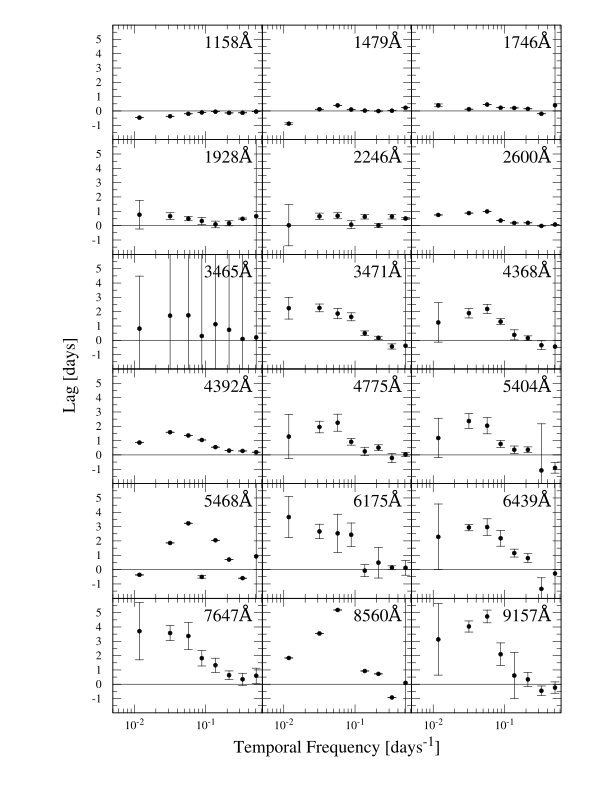
\includegraphics[width=.9\textwidth]{../img/timelag_atlas.pdf}
        \caption{Time delays for all observed light curves relative to 1367\AA. The delay increases with wavelength, as predicted by the accretion disk model. These functions can ultimately be used to reconstruct the transfer function.}
        \label{timelag_atlas}
    \end{figure}

\section{Discussion}

Frequency-dependent power spectral densities confirm time-dependent variability in the emission strengths for each band. This  This behaviour is expected for any active galactic nucleus and has been long-confirmed in NGC 5548, so it comes as no surprise to find those results here.

Analysis of the top-hat impulse response model predicted frequency-dependent time delays, which have been recovered from the light curves in this analysis. Furthermore, the distribution of time delays indicates a wavelength-dependent nature. This warrants further study and analysis.

\begin{figure}
    \centering
    \begin{minipage}{.475\textwidth}
        \centering
        \includegraphics[width=1\linewidth]{../img/tophat_freqdomain.pdf}
        \captionof{figure}{Time delays modeled from tophat impulse responses.}
        \label{fig:top_freq_comp}
    \end{minipage}
    \hfill
    \begin{minipage}{.475\textwidth}
        \centering
        \includegraphics[width=1\linewidth]{../img/timelag_1367Å_≺_7647Å_{σ∊CM}.pdf}
        \captionof{figure}{The time delay computed from the cross spectrum of 7647\AA and 1367\AA.}
        \label{fig:timelag_comp}
    \end{minipage}
\end{figure}

The analyses performed on these data have elucidated clear trends in the PSD and time delays. With reverberation mapping, the goal is to recover the transfer function, which encodes the geometry of the system. Recovering the time delays is a significant step toward that goal.

%\bsp
\bibliographystyle{plainnat}
\bibliography{wsu_reu}



\end{document}